%
% jordan.tex
%
% (c) 2021 Prof Dr Andreas Müller, OST Ostschweizer Fachhochschule
%
\bgroup

\definecolor{darkgreen}{rgb}{0,0.6,0}
\def\L#1{
	\node at ({#1-0.5},{0.5-#1}) {$\lambda$};
}
\def\E#1{
	\node at ({#1-0.5},{1.5-#1}) {$1$};
}

\begin{frame}[t]
\frametitle{Jordan Normalform}
\vspace{-15pt}
\begin{columns}[t,onlytextwidth]
\begin{column}{0.40\textwidth}
\begin{block}{Wahl der Basis}
\begin{enumerate}
\item<2-> Zerlegung in verallgemeinerte Eigenräume
\begin{align*}
V
&=
\mathcal{E}_{{\color{blue}\lambda}}(A)
\oplus
\mathcal{E}_{{\color{darkgreen}\lambda}}(A)
\oplus
\mathcal{E}_{{\color{red}\lambda}}(A)
%\oplus
%\dots
\\
\llap{$A\mathcal{E}_{{\color{blue}\lambda}}$}(A)
&\subset
\mathcal{E}_{{\color{blue}\lambda}}(A)
\\
\llap{$A\mathcal{E}_{{\color{darkgreen}\lambda}}$}(A)
&\subset
\mathcal{E}_{{\color{darkgreen}\lambda}}(A)
\\
\llap{$A\mathcal{E}_{{\color{red}\lambda}}$}(A)
&\subset
\mathcal{E}_{{\color{red}\lambda}}(A),
\dots
\end{align*}
\item<3-> In jedem Eigenraum: Zerlegung in Jordan-Blöcke
\end{enumerate}
\end{block}
\end{column}
\begin{column}{0.56\textwidth}
\begin{center}
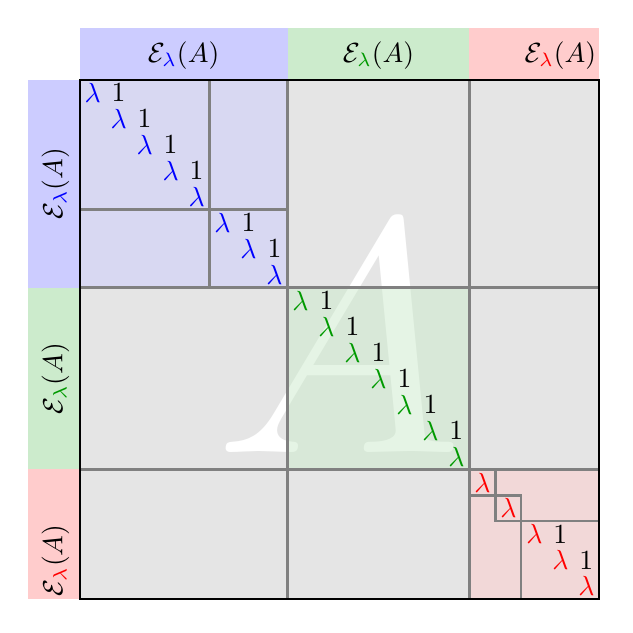
\begin{tikzpicture}[>=latex,thick,scale=0.33]
\fill[color=gray!20] (0,-20) rectangle (20,0);
\node[color=white] at (10,-10) [scale=12] {$A$};

\uncover<2->{
	\fill[color=blue!20,opacity=0.5] (0,0) rectangle (8,-8);
	\fill[color=darkgreen!20,opacity=0.5] (8,-8) rectangle (15,-15);
	\fill[color=red!20,opacity=0.5] (15,-15) rectangle (20,-20);
	\fill[color=blue!20] (0,0) rectangle (8,2);
	\fill[color=blue!20] (-2,-8) rectangle (0,0);
	\fill[color=darkgreen!20] (8,0) rectangle (15,2);
	\fill[color=darkgreen!20] (-2,-15) rectangle (0,-8);
	\fill[color=red!20] (15,0) rectangle (20,2);
	\fill[color=red!20] (-2,-20) rectangle (0,-15);
}

\uncover<3->{
	\draw[color=gray] (0,0) rectangle (5,-5);
	\draw[color=gray] (5,-5) rectangle (8,-8);
	\draw[color=gray] (8,-8) rectangle (15,-15);
	\draw[color=gray] (15,-15) rectangle (16,-16);
	\draw[color=gray] (16,-16) rectangle (17,-17);
	\draw[color=gray] (17,-17) rectangle (20,-20);
}

\uncover<2->{
	\draw[color=gray] (8,0) -- (8,-20);
	\draw[color=gray] (15,0) -- (15,-20);
	\draw[color=gray] (0,-8) -- (20,-8);
	\draw[color=gray] (0,-15) -- (20,-15);

	\node at (0,-4) [above,rotate=90]
		{$\mathcal{E}_{{\color{blue}\lambda}}(A)$};
	\node at (4,0) [above]
		{$\mathcal{E}_{{\color{blue}\lambda}}(A)$};
	\node at (0,-11.5) [above,rotate=90]
		{$\mathcal{E}_{{\color{darkgreen}\lambda}}(A)$};
	\node at (11.5,0) [above]
		{$\mathcal{E}_{{\color{darkgreen}\lambda}}(A)$};
	\node at (0,-18.5) [above,rotate=90]
		{$\mathcal{E}_{{\color{red}\lambda}}(A)$};
	\node at (18.5,0) [above]
		{$\mathcal{E}_{{\color{red}\lambda}}(A)$};
}

\uncover<2->{
	{\color{blue}
	\foreach \x in {1,...,8}{ \L{\x} }
	}
	{\color{darkgreen}
	\foreach \x in {9,...,15}{ \L{\x} }
	}
	{\color{red}
	\foreach \x in {16,...,20}{ \L{\x} }
	}
}

\uncover<3->{
\E{2}
\E{3}
\E{4}
\E{5}

\E{7}
\E{8}

\E{10}
\E{11}
\E{12}
\E{13}
\E{14}
\E{15}

\E{19}
\E{20}
}

\draw (0,-20) rectangle (20,0);
\end{tikzpicture}
\end{center}
\end{column}
\end{columns}
\end{frame}

\egroup
